
\documentclass[14pt]{beamer}

%%%%%%%%%%%%%%%%%%%%%%%%%%%%%%%%%%%%%%%%%%%%%%%%%%%%%%%%%%%%%%%%%%%%%%%%%%%%%%%%

    \usepackage{fix-cm}
    \usepackage[english]{babel}
    \usepackage[utf8]{inputenc}
    \usepackage[T1]{fontenc}
    \usepackage{lmodern}
    \usepackage{textcomp}
    \usepackage[cm]{sfmath}
    \usepackage[euler]{textgreek}
    \usepackage{xfrac}
    \mathchardef\mhyphen="2D
    \usepackage{multirow}
    \usepackage{tikz}
    \usetikzlibrary{arrows,calc}
    \usepackage{bbding}
    \usepackage{xcolor}

    %% Set the left and right margins
    \setbeamersize{text margin left=1em,text margin right=1em}

    %% Fonts
    \setbeamerfont{title}{series=\bfseries,size=\huge}
    \setbeamerfont{subtitle}{series=\bfseries,size=\large}
    \setbeamerfont{date}{size=\footnotesize}
    \setbeamerfont{frametitle}{series=\bfseries,size=\large}
    \setbeamerfont{block title}{series=\bfseries,size=\large}
    \setbeamerfont{footline}{size=\normalsize}

    %% Colors
    %\setbeamercolor{background canvas}{bg=white!5!black}    % Blackboard
    %\setbeamercolor{structure}{fg=white!97.5!black}         % Chalk
    \setbeamercolor{background canvas}{bg=black!0!white}         % Chalk
    \setbeamercolor{structure}{fg=white!5!black}    % Blackboard
    \usebeamercolor{structure}
    \setbeamercolor{normal text}{fg=structure.fg}

    %% Add a line after the frametitle
    \setbeamertemplate{frametitle}[default][left,leftskip=1ex]
    \addtobeamertemplate{frametitle}{}{\vspace*{-1ex}\rule{\textwidth}{2pt}}

    %% Use circular discs as itemized list markers
    \setbeamertemplate{itemize items}[circle]

    %% Remove default navigation symbols
    \setbeamertemplate{navigation symbols}{}

    %% Remove the footline
    \setbeamertemplate{footline}{}

    % MMACa Logo
    \setlength{\fboxsep}{3pt}
    \setlength{\fboxrule}{0.75pt}

    \definecolor{GREEN}{RGB}{18, 159, 87}


%%%%%%%%%%%%%%%%%%%%%%%%%%%%%%%%%%%%%%%%%%%%%%%%%%%%%%%%%%%%%%%%%%%%%%%%%%%%%%%%

\title{\Huge Spira Mirabilis\\[-1.2ex]}
\author{{\large \href{https://github.com/CarlosLunaMota}{Carlos Luna Mota}}\\[2ex]
        \includegraphics[width=22ex, angle=90]{pictures/Spiral_Phi_90.pdf}\\[-5ex]}
\date{\href{https://mmaca.cat/}{\includegraphics[scale=0.1]{pictures/MMACA.png}}}


\begin{document}

    %%%%%%%%%%%%%%%%%%%%%%%%%%%%%%%%%%%%%%%%%%%%%%%%%%%%%%%%%%%%%%%%%%%%%%%%%%%%

    \begin{frame}
      \titlepage
    \end{frame}

    %%%%%%%%%%%%%%%%%%%%%%%%%%%%%%%%%%%%%%%%%%%%%%%%%%%%%%%%%%%%%%%%%%%%%%%%%%%%

    \begin{frame}{}
        \begin{center}
            \textbf{\Large Maths are useful...}

            \bigskip \bigskip \bigskip \bigskip
            
            \textbf{\Huge So what?}
        \end{center}
    \end{frame}

    %%%%%%%%%%%%%%%%%%%%%%%%%%%%%%%%%%%%%%%%%%%%%%%%%%%%%%%%%%%%%%%%%%%%%%%%%%%%

    \begin{frame}{}
        \begin{center}
            {\large \textbf{Amazement} $\Rightarrow$ \textbf{Engagement} $\Rightarrow$ \textbf{Joy}}

            {\LARGE \bigskip \bigskip \bigskip \bigskip

            {Maths should be exciting!}}
        \end{center}
    \end{frame}

    %%%%%%%%%%%%%%%%%%%%%%%%%%%%%%%%%%%%%%%%%%%%%%%%%%%%%%%%%%%%%%%%%%%%%%%%%%%%

    {
    \usebackgroundtemplate{\includegraphics[width=\paperwidth]{pictures/Compas.jpg}}
    \begin{frame}[plain]
    \end{frame}
    }

    %%%%%%%%%%%%%%%%%%%%%%%%%%%%%%%%%%%%%%%%%%%%%%%%%%%%%%%%%%%%%%%%%%%%%%%%%%%%

    {
    \usebackgroundtemplate{\includegraphics[width=\paperwidth]{pictures/Escarbat.jpg}}
    \begin{frame}[plain]
    \end{frame}
    }

    %%%%%%%%%%%%%%%%%%%%%%%%%%%%%%%%%%%%%%%%%%%%%%%%%%%%%%%%%%%%%%%%%%%%%%%%%%%%

    {
    \usebackgroundtemplate{\includegraphics[width=\paperwidth]{pictures/Atenes 2.jpg}}
    \begin{frame}[plain]
    \end{frame}
    }

    %%%%%%%%%%%%%%%%%%%%%%%%%%%%%%%%%%%%%%%%%%%%%%%%%%%%%%%%%%%%%%%%%%%%%%%%%%%%
    
    {
    \usebackgroundtemplate{\includegraphics[width=\paperwidth]{pictures/Atenes 1.jpg}}
    \begin{frame}[plain]
    \end{frame}
    }

    %%%%%%%%%%%%%%%%%%%%%%%%%%%%%%%%%%%%%%%%%%%%%%%%%%%%%%%%%%%%%%%%%%%%%%%%%%%%
    
    %{
    %\usebackgroundtemplate{\includegraphics[width=\paperwidth]{pictures/Janvier.jpg}}
    %\begin{frame}[plain]
    %\end{frame}
    %}

    %%%%%%%%%%%%%%%%%%%%%%%%%%%%%%%%%%%%%%%%%%%%%%%%%%%%%%%%%%%%%%%%%%%%%%%%%%%%

    \begin{frame}{A perfect STEAM project!}
        \begin{center}
            \vspace{-1em}
            \begin{minipage}{12ex}
                \includegraphics[height=30ex]{pictures/Funcionament Compas Auri.jpg}
            \end{minipage} \qquad \begin{minipage}{20ex}
                 \large \phantom{.}\\[2ex]
                 \begin{tabular}{ll}
                    \textbf{S}cience & {\color{GREEN}\textbf{\Checkmark}}\\[1ex]
                    \textbf{T}echnology & {\color{GREEN}\textbf{\Checkmark}}\\[1ex]
                    \textbf{E}ngineering & {\color{GREEN}\textbf{\Checkmark}}\\[1ex]
                    \textbf{A}rt & {\color{GREEN}\textbf{\Checkmark}}\\[1ex]
                    \textbf{M}aths & {\color{GREEN}\textbf{\Checkmark}}\\[1ex]
                \end{tabular}
            \end{minipage}

            \bigskip
            
            {\small In too many STEAM projects... {The M is silent!}}
        \end{center}
    \end{frame}

    %%%%%%%%%%%%%%%%%%%%%%%%%%%%%%%%%%%%%%%%%%%%%%%%%%%%%%%%%%%%%%%%%%%%%%%%%%%%

    \begin{frame}{}
        \begin{center}
            \textbf{\Huge But...}
        \end{center}
    \end{frame}

    %%%%%%%%%%%%%%%%%%%%%%%%%%%%%%%%%%%%%%%%%%%%%%%%%%%%%%%%%%%%%%%%%%%%%%%%%%%%

    {
    \usebackgroundtemplate{\includegraphics[width=\paperwidth]{pictures/Targetes.jpg}}
    \begin{frame}[plain]
    \end{frame}
    }

    %%%%%%%%%%%%%%%%%%%%%%%%%%%%%%%%%%%%%%%%%%%%%%%%%%%%%%%%%%%%%%%%%%%%%%%%%%%%    

    \begin{frame}{The solution that amazed... no one}
        \begin{center}
            \includegraphics[height=30ex]{pictures/Rectangle.jpg}
        \end{center}
    \end{frame}

    %%%%%%%%%%%%%%%%%%%%%%%%%%%%%%%%%%%%%%%%%%%%%%%%%%%%%%%%%%%%%%%%%%%%%%%%%%%%    

    \begin{frame}{Analog computers}
        \begin{center}
            \includegraphics[height=20ex]{pictures/Monkey.jpg}
            \includegraphics[height=20ex]{pictures/Sector.png}

            \bigskip

            \includegraphics[height=10ex]{pictures/Slide.jpg}
        \end{center}
    \end{frame}

    %%%%%%%%%%%%%%%%%%%%%%%%%%%%%%%%%%%%%%%%%%%%%%%%%%%%%%%%%%%%%%%%%%%%%%%%%%%%    

    \begin{frame}{Nomograms}
        \bigskip
        \!\!\!\!\!\!\includegraphics[width=\paperwidth]{pictures/Nomogram.jpg}
    \end{frame}

    %%%%%%%%%%%%%%%%%%%%%%%%%%%%%%%%%%%%%%%%%%%%%%%%%%%%%%%%%%%%%%%%%%%%%%%%%%%%    

    \begin{frame}{Two spirals that compute!}
        \begin{center}
            \begin{tabular}{cccc}
                \textbf{Archimedean} & \qquad & \textbf{Logarithmic} & \quad \\[1ex]
                \includegraphics[width=20ex]{pictures/Arquimedes.jpg} & & 
                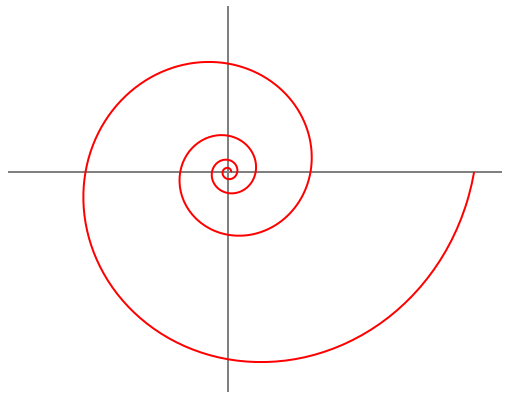
\includegraphics[width=20ex]{pictures/Logaritmica.jpg} & \\[1ex]
                {\Large $r = \lambda\cdot\alpha$ } & & {\Large $r = \lambda^\alpha$ } & \\
            \end{tabular}
        \end{center}
    \end{frame}

    %%%%%%%%%%%%%%%%%%%%%%%%%%%%%%%%%%%%%%%%%%%%%%%%%%%%%%%%%%%%%%%%%%%%%%%%%%%%    

    \begin{frame}{Two spirals that compute!}
        \begin{center}
            \begin{tabular}{cccc}
                \textbf{Archimedean} & \qquad & \textbf{Logarithmic} & \quad \\[1ex]
                \includegraphics[width=20ex]{pictures/Yoga.jpg} & &
                \includegraphics[width=20ex]{pictures/Nautilus.jpg} & \\[1ex]
                {\Large $r = \lambda\cdot\alpha$ } & & {\Large $r = \lambda^\alpha$ } & \\
            \end{tabular}
        \end{center}
    \end{frame}

    %%%%%%%%%%%%%%%%%%%%%%%%%%%%%%%%%%%%%%%%%%%%%%%%%%%%%%%%%%%%%%%%%%%%%%%%%%%%    

    \begin{frame}{Spira Mirabilis!}
        \begin{center}
            \begin{minipage}{20ex}
                \includegraphics[height=32ex]{pictures/Spiral_Phi_90.pdf}
            \end{minipage} \begin{minipage}{29ex}
                \textbf{\large \quad History:}
                \bigskip
                \begin{itemize}
                    \small
                    \item Described by \textbf{Albrecht Dürer} (1525)\\[2ex]
                    \item Studied by \textbf{René Descartes} (1638) \\[2ex]
                    \item Named \emph{Spira Mirabilis} by \textbf{Jakob Bernoulli} (1692)
                \end{itemize}
            \end{minipage}            
        \end{center}
    \end{frame}

    %%%%%%%%%%%%%%%%%%%%%%%%%%%%%%%%%%%%%%%%%%%%%%%%%%%%%%%%%%%%%%%%%%%%%%%%%%%%    

    \begin{frame}{Spira Mirabilis!}
        \begin{center}
            \begin{minipage}{20ex}
                \includegraphics[height=32ex]{pictures/Spiral_Phi_90.pdf}
            \end{minipage} \begin{minipage}{29ex}
                \textbf{\large \quad Properties:}
                \bigskip
                \begin{itemize}
                    \small
                    \item It has a \textbf{center},\\ but never reaches it!\\[2ex]
                    \item It maintains a \textbf{constant angle}\\ between tangents and radii\\[2ex]
                    \item \textbf{Rotating} = \textbf{Scaling}
                \end{itemize}
                \bigskip
            \end{minipage}            
        \end{center}
    \end{frame}

    %%%%%%%%%%%%%%%%%%%%%%%%%%%%%%%%%%%%%%%%%%%%%%%%%%%%%%%%%%%%%%%%%%%%%%%%%%%%    

    {
    \usebackgroundtemplate{\includegraphics[width=\paperwidth]{pictures/Tomba.jpg}}
    \begin{frame}[plain]
    \end{frame}
    }

    %%%%%%%%%%%%%%%%%%%%%%%%%%%%%%%%%%%%%%%%%%%%%%%%%%%%%%%%%%%%%%%%%%%%%%%%%%%%    
    
    \begin{frame}{Spira Mirabilis!}
        \begin{center}
            \vspace{-2ex}
            \includegraphics[width=32ex, angle=90]{pictures/Spiral_Phi_90.pdf}
        \end{center}
    \end{frame}
    
    %%%%%%%%%%%%%%%%%%%%%%%%%%%%%%%%%%%%%%%%%%%%%%%%%%%%%%%%%%%%%%%%%%%%%%%%%%%%    
    
    \begin{frame}{The\; $\phi\;/\;180^\circ$\; and\; $\phi\;/\;360^\circ$ spirals}
        \begin{center}
            \includegraphics[height=34ex]{pictures/Example_1.pdf}\quad
            \includegraphics[height=34ex]{pictures/Example_2.pdf}
        \end{center}
    \end{frame}

    %%%%%%%%%%%%%%%%%%%%%%%%%%%%%%%%%%%%%%%%%%%%%%%%%%%%%%%%%%%%%%%%%%%%%%%%%%%%    

    \begin{frame}{The\; $\phi\;/\;90^\circ\phantom{1}$\; and\; $\phi\;/\;270^\circ$ spirals}
        \begin{center}
            \includegraphics[height=34ex]{pictures/Example_3.pdf}\quad
            \includegraphics[height=34ex]{pictures/Example_4.pdf}
        \end{center}
    \end{frame}

    %%%%%%%%%%%%%%%%%%%%%%%%%%%%%%%%%%%%%%%%%%%%%%%%%%%%%%%%%%%%%%%%%%%%%%%%%%%%    

    \begin{frame}{Fibonacci Spiral $\;\approx\;$ the\; $\phi\;/\;90^\circ$ spiral}
        \begin{center}
            \includegraphics[width=34ex, angle=90]{pictures/Example_5.pdf}
        \end{center}
    \end{frame}

    %%%%%%%%%%%%%%%%%%%%%%%%%%%%%%%%%%%%%%%%%%%%%%%%%%%%%%%%%%%%%%%%%%%%%%%%%%%%    

    \begin{frame}{The\; $\sqrt{2}\;/\;270^\circ$\; and\; $\sqrt{3}\;/\;270^\circ$ spirals}
        \begin{center}
            \includegraphics[height=34ex]{pictures/Example_6.pdf}\quad
            \includegraphics[height=34ex]{pictures/Example_7.pdf}
        \end{center}
    \end{frame}

    %%%%%%%%%%%%%%%%%%%%%%%%%%%%%%%%%%%%%%%%%%%%%%%%%%%%%%%%%%%%%%%%%%%%%%%%%%%%    
    
    \begin{frame}{\;\; $\sqrt{2}\;/\;90^\circ \quad=\quad 2\;/\;180^\circ \quad=\quad 4\;/\;360^\circ$}
        \begin{center}
            \includegraphics[height=24ex]{pictures/Spiral_Root2_090.pdf}
            
\includegraphics[height=24ex]{pictures/Spiral_2_180.pdf}
            \includegraphics[height=24ex]{pictures/Spiral_4_360.pdf}
        \end{center}
    \end{frame}

    %%%%%%%%%%%%%%%%%%%%%%%%%%%%%%%%%%%%%%%%%%%%%%%%%%%%%%%%%%%%%%%%%%%%%%%%%%%%    
    
    \begin{frame}{Doubling the cube with the\, $2\;/\;270^\circ$ spiral}
        \begin{center}
            \begin{minipage}{25ex}
                \includegraphics[height=34ex]{pictures/Example_8.pdf}
            \end{minipage} \begin{minipage}{25ex}
                \includegraphics[height=15ex]{pictures/Doubling Cube.png}
            \end{minipage}
        \end{center}
    \end{frame}
    
    %%%%%%%%%%%%%%%%%%%%%%%%%%%%%%%%%%%%%%%%%%%%%%%%%%%%%%%%%%%%%%%%%%%%%%%%%%%%    

    \begin{frame}{}
        \begin{center}
            \textbf{\Large Thank you for your attention!\\[1ex]Any questions?}

            \bigskip \bigskip

            \href{https://github.com/CarlosLunaMota/Spira-Mirabilis}{\includegraphics[height=16ex]{pictures/QR.png}} \qquad \quad \href{https://mmaca.cat/}{\includegraphics[height=16ex]{pictures/MMACA_10.jpeg}}

            \bigskip \bigskip
            
            \href{https://github.com/CarlosLunaMota/Spira-Mirabilis}{https://github.com/CarlosLunaMota/Spira-Mirabilis}
        \end{center}
    \end{frame}
    
\end{document}
